\subsection{Functions}

\begin{tcolorbox}[title=Problem 1, breakable]
    (a) Let $A = \{1, 2, 3\}, B = \{4\}$, and 
        $f = \{(1, 4), (2, 4), (3, 4)\}$.
        Is $f$ a function from $A$ to $B$?

    (b) Let $A = \{1\}, B = \{2, 3, 4\}$ and
        $f = \{(1, 2), (1, 3), (1, 4)\}$.
        Is $f$ a function from $A$ to $B$.

    (c) Let $C$ be the set of all cars registered
        in your state, and let $S$ be the set of all
        finite sequences of letters and digits.
        Let $L = \{(c, s) \in C \times S \mid 
            \text{the license plate number of the car $c$ is $s$}\}$.
        Is $L$ a function from $C$ to $S$.
\end{tcolorbox}

\textbf{Solution (a):}

Yes.

\textbf{Solution (b):}

No.

\textbf{Solution (c):}

Yes.

\begin{tcolorbox}[title=Problem 2, breakable]
    (a) Let $f$ be the relation represented by the graph in Figure $5.3$.
        Is $f$ a function from $A$ to $B$.

    (b) Let $W$ be the set of all words of English, and let $A$ be the set 
        of all letters of the alphabet. 
        Let 
        \[f = \{(w, a) \in W \times A \mid \text{the letter $a$ occurs in the word $w$}\}\]
        and let 
        \[g = \{(w, a) \in W \times A \mid \text{the letter $a$ is the first letter of the word $w$}\}\]
        Is $f$ a function from $W$ to $A$?
        How about $g$?

    (c) John, Mary, Susan, and Fred go out to dinner and sit at a round table.
        Let 
        \[P = \{\text{John, Mary, Susan, Fred}\}\]
        and let 
        \[R = \{(p, q) \in P \times P \mid \text{the person $p$ is sitting immediately to the right of person $q$}\}\]
        Is $R$ a function from $P$ to $P$.
\end{tcolorbox}

\begin{figure}[h]
    \centering
    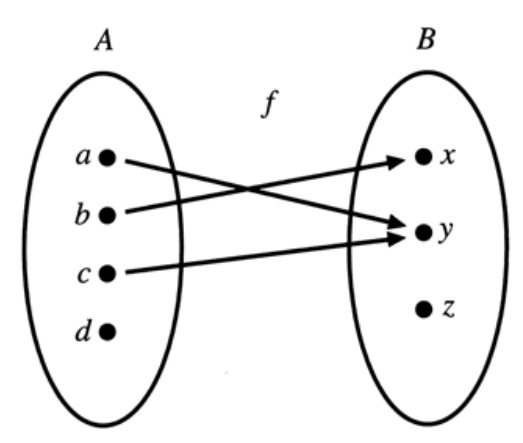
\includegraphics[width=0.4\textwidth]{images/func.png}
\end{figure}

\textbf{Solution (a):}

No.

\textbf{Solution (b):}

$f$: No.
$g$: Yes.

\textbf{Solution (c):}

Yes.

\begin{tcolorbox}[title=Problem 7, breakable]
    Suppose $f : A \rightarrow B$ and $C \subseteq A$.
    The set $f \cap (C \times B)$, which is a relation from $C$ to $B$,
        is called the \emph{restriction} of $f$ to $C$, and is sometimes
        denoted $f | C$. 
    In other words.\
    \[f | C = f \cap (C \times B)\]
    (a) Prove that $f | C$ is a function from $C$ to $B$ and that for all $c \in C$,
        $f(c) = (f | C)(c)$.

    (b) Suppose $g : C \rightarrow B$. Prove that $g = f | C$ iff $g \subseteq f$.

    (c) Let $g$ and $h$ be the functions defined in parts $2$ and $3$ of Example $5.1.3$.
        Show that $g = h | \mathbb{Z}$.
        \[g : \mathbb{Z} \rightarrow \mathbb{R} \text{ and } g(x) = 2x + 3\]
        \[h : \mathbb{R} \rightarrow \mathbb{R} \text{ and } h(x) = 2x + 3\]
\end{tcolorbox}

\begin{proof}
    We must show that $f|C$ is a function.  
    For all $x \in C$, there exists $y$ such that $(x, y) \in f|C$,  
    and there is exactly one $y \in B$ such that $(x, y) \in f|C$.

    Let $x$ be an arbitrary element in $C$.
    Since $C \subseteq A$, it follows that $x \in A$.
    Since $f$ is a function from $A$ to $B$, 
        there exists $y \in B$ such that $(x, y) \in f$.
    Clearly, $(x, y) \in A \times B$.
    Since $(x, y) \in f$ and $(x, y) \in C \times B$,
        it follows that $(x, y) \in f \cap (C \times B) = f|C$.
    Thus $f|C$ maps all elements in $C$ to $B$.

    Notice that $f \cap (C \times B) \subseteq f$.
    Then, since $(x, y) \in f|C$, it follows that $(x, y) \in f$.
    It follows that, since $f$ is a function, 
        $x$ maps to exactly one element in $B$, namely $y$.
\end{proof}

\begin{proof}
    Suppose $g : C \rightarrow B$.

    ($\rightarrow$) Suppose $g = f|C$.
    Then $g = f|C = f \cap (C \times B) \subseteq f$.

    ($\leftarrow$) Suppose $g \subseteq f$.
    Let $(x, y)$ be an arbitrary element in $g$.
    Since $g \subseteq f$, it follows that $(x, y) \in f$.
    Since $(x, y) \in g$, it follows that $(x, y) \in C \times B$.
    Thus $(x, y) \in f$ and $(x, y) \in C \times B$.
    Therefore $(x, y) \in f \cap (C \times B) = f|C$.
    It follows that $g \subseteq f|C$.

    Let $(x, y)$ be an arbitrary element in $f|C$.
    It follows that $(x, y) \in f$ and $(x, y) \in C \times B$.
    Since $g \subseteq f$ and $x \in C$, it follows that $(x, y) \in g$.
    Thus $f|C \subseteq g$.
\end{proof}

\begin{proof}
    We need to show that $g = h|\mathbb{Z} = h \cap (\mathbb{Z} \times \mathbb{R})$.
    
    Suppose $(x, y)$ is an arbitrary element in $g$.
    We know that $(x, y) \in \mathbb{Z} \times \mathbb{R}$.
    It follows that $x \in \mathbb{Z}$ and $y \in \mathbb{R}$.
    Since $\mathbb{Z} \subseteq \mathbb{R}$, it follows that $x \in \mathbb{R}$.
    Therefore $(x, y) \in h$.
    Since $(x, y) \in h$ and $(x, y) \in \mathbb{Z} \times \mathbb{R}$,
        it follows that $(x, y) \in h|\mathbb{Z}$.
    Thus $g \subseteq h|\mathbb{Z}$.

    Suppose $(x, y)$ is an arbitrary element in $h|\mathbb{Z}$.
    It follows that $(x, y) \in h$ and $(x, y) \in \mathbb{Z} \times \mathbb{R}$.
    Since $x \in \mathbb{Z}$, it follows that $(x, y) \in g$.
    Thus $h|\mathbb{Z} \subseteq g$.
\end{proof}

\begin{tcolorbox}[title=Problem 8, breakable]
    Suppose $f : A \rightarrow B$ and $g \subseteq f$.
    Prove that there is a set $A' \subseteq A$ such that 
        $g : A' \rightarrow B$.
\end{tcolorbox}

\begin{proof}
    Let $A' = dom(g)$.
    It is clear that $A' \subseteq A$,
        since $dom(g) \subseteq dom(f)$.
    Let $x \in A'$. Then there exists $y$ such that $(x, y) \in g$.
    Since $g \subseteq f$, it follows that $(x, y) \in f$.
    There is only a single element that $x$ maps to,
        since $g \subseteq f$ and $f$ is a function.
    Thus $g : A' \rightarrow B$.
\end{proof}

\begin{tcolorbox}[title=Problem 9, breakable]
    Suppose $f : A \rightarrow B$, $B \ne \emptyset$, and $A \subseteq A'$.
    Prove that there is a function $g : A' \rightarrow B$ such that $f \subseteq g$.
\end{tcolorbox}

\begin{proof}
    Let $A'' = A' \setminus A$.
    Since $B \ne \emptyset$, let $y$ be an element in $B$.
    Let $g = f \cup \{(x, y) \mid x \in A''\}$.
    Then for each $x \in A$ there is a unique $y$ such that $(x, y) \in f$,
    and for each $x \in A''$ there is exactly one pair $(x, y)$ in $g$.
    Thus $g$ is a function from $A'$ to $B$ and $f \subseteq g$.
\end{proof}

\newpage
\begin{tcolorbox}[title=Problem 11, breakable]\
    Suppose $A$ is a set. 
    Show that $i_A$ is the only relation on $A$ that 
        is both an equivalence relation and also a function from $A$ to $A$.
\end{tcolorbox}

\begin{proof}
    For contradiction, suppose $R \ne i_A$ is an equivalence relation on $A$
        and $R : A \rightarrow A$.
    Then there exists a pair $(x, y) \in R$ such that $x \ne y$.
    Since $R$ is reflexive, $(x, x) \in R$.
    Thus $R$ contains both $(x, x)$ and $(x, y)$ with $y \ne x$,
        contradicting that $R$ is a function.
    Therefore $R = i_A$.
\end{proof}

\begin{tcolorbox}[title=Problem 12, breakable]
    Suppose $f : A \rightarrow C$ and $g : B \rightarrow C$.

    (a) Prove that if $A$ and $B$ are disjoint, then $f \cup g : A \cup B \rightarrow C$.

    (b) Prove that $f \cup g : A \cup B \rightarrow C$ iff $f | (A \cap B) = g | (A \cap B)$.
        (See excersize $7$ for the meaning of the notation used here.)
\end{tcolorbox}

\begin{proof}
    Suppose $A$ and $B$ are disjoint.
    Let $x$ be an arbitrary element in $A \cup B$.
    Either $x \in A$ or $x \in B$.
    If $x \in A$, then under $f$ there exists a unique $y \in C$
        such that $(x, y) \in f$.
    If $x \in B$, then under $g$ there exists a unique $y \in C$
        such that $(x, y) \in g$.
    Since $A$ and $B$ are disjoint, $f \cup g$ assigns exactly one $y \in C$
        to each $x \in A \cup B$.
    Therefore $f \cup g : A \cup B \rightarrow C$.
\end{proof}

\begin{proof}
    ($\rightarrow$) Suppose $f \cup g : A \cup B \rightarrow C$.
    For contradiction assume $f | (A \cap B) \ne g | (A \cap B)$.
    Suppose w.l.o.g. since $f | (A \cap B) \ne g | (A \cap B)$
        there is a pair $(x, y) \in f | (A \cap B)$
        such that $(x, y) \notin g | (A \cap B)$.
    Now clearly $(x, y) \in f$, but since $g$ is a function on $B$
        and $x \in A \cap B$, there is a pair $(x, y') \in g$.
    Thus $f \cup g$ results in two mappings from $x$ to $y$ and $y'$,
    which contradicts that $f \cup g$ is a function.
    Therefore, $f | (A \cap B) = g | (A \cap B)$.

    ($\leftarrow$) Suppose $f | (A \cap B) = g | (A \cap B)$.
    We must show that $f \cup g : A \cup B \rightarrow C$.
    Let $(x, y)$ and $(x, y')$ be elements of $f \cup g$.
    We need to show $y = y'$.
    If both pairs are in $f$ or both in $g$, this follows since
    $f$ and $g$ are functions.
    If one pair is from $f$ and the other from $g$, then
    $x \in A \cap B$ and hence $(x, y) \in f | (A \cap B)$
    and $(x, y') \in g | (A \cap B)$.
    By assumption $f | (A \cap B) = g | (A \cap B)$, so $y = y'$.
    Thus $f \cup g$ is a function from $A \cup B$ to $C$.
\end{proof}

\begin{tcolorbox}[title=Problem 13, breakable]
    Suppose $R$ is a relation from $A$ to $B$, $S$ is a relation 
    from $B$ to $C$, $Ran(R) = Dom(S) = B$, and $S \circ R : A \rightarrow C$.

    (a) Prove that $S : B \rightarrow C$.

    (b) Give an example to show that it need not be the case 
        that $R : A \rightarrow B$.
\end{tcolorbox}

\begin{proof}
    Let $b$ be an arbitrary element in $B$.
    Since $Ran(R) = Dom(S) = B$, there exists $a \in A$ such that $(a, b) \in R$.
    Because $S \circ R$ is a function, there is exactly one $c \in C$
        such that $(a, c) \in S \circ R$.
    By the definition of composition, this means $(a, b) \in R$ and $(b, c) \in S$.
    Thus $S$ maps $b$ to a unique $c \in C$.
    Therefore, $S : B \rightarrow C$.
\end{proof}

\textbf{Solution (b):}
\[R = \{(1, 2), (1, 3)\}, S = \{(2, 4), (3, 4)\}, S \circ R = \{(1, 4)\}\]

\newpage
\begin{tcolorbox}[title=Problem 17, breakable]
    Suppose $A$ is a nonempty set and $f : A \rightarrow A$.

    (a) Suppose there is some $a \in A$ such that 
        $\forall{x} \in A(f(x) = a)$. (In this case, $f$ is called 
        a constant function.) Prove that for all $g : A \rightarrow A$,
        $f \circ g  = f$.

    (b) Suppose that for all $g : A \rightarrow A$, $f \circ g = f$.
        Prove that $f$ is a constant function. (Hint: what happens
        if $g$ is a constant function?)
\end{tcolorbox}

\begin{proof}
    Let $(x, z)$ be an arbitrary pair in $f \circ g$.
    There exists $y$ such that $(x, y) \in g$ and $(y, z) \in f$.
    It follows, since $f$ is a constant function, that $(x, z) \in f$.
    Thus $f \circ g \subseteq f$.

    Let $(x, z)$ be an arbitrary pair in $f$.
    Now, since $g : A \rightarrow A$ is a function, for this $x \in A$
        there exists a unique $y \in A$ such that $(x, y) \in g$.
    Since $f$ is a constant function and $y \in A$,
        it follows that $(y, z) \in f$.
    Since $(x, y) \in g$ and $(y, z) \in f$, 
        it follows that $(x, z) \in f \circ g$.
    Thus $f \subseteq f \circ g$.

    Therefore $f \circ g = f$.
\end{proof}

\begin{proof}
    Let $x_0 \in A$ and define 
        $g : A \to A$ such that $g(x) = x_0$ for all $x \in A$.
    Then for every $x \in A$, $(f \circ g)(x) = f(g(x)) = f(x_0)$.
    By assumption, $f \circ g = f$, so for every $x \in A$, $f(x) = (f \circ g)(x) = f(x_0)$.
    Therefore, $f$ maps every element of $A$ to the same value.
    It follows that $f$ is a constant function.
\end{proof}

\begin{tcolorbox}[title=Problem 19, breakable]
    Let $\mathcal{F} = \{f \mid f : \mathbb{Z}^+ \rightarrow \mathbb{R}\}$.
    For $g \in \mathcal{F}$, we define the set $O(g)$ as follows:
    \[O(g) = \{f \in \mathcal{F} \mid \exists{a} \in \mathbb{Z}^+
                \exists{c} \in \mathbb{R}^+ \forall{x} > a (|f(x)| \le c|g(x)|)\}\]
    (If $f \in O(g)$, then mathematicians say ``$f$ is big-oh of $g$''.)

    (a) Let $f : \mathbb{Z}^+ \rightarrow \mathbb{R}$ and $g : \mathbb{Z}^+ \rightarrow \mathbb{R}$
        be defined by the formulas $f(x) = 7x + 3$ and $g(x) = x^2$. 
        Prove that $f \in O(g)$, but $g \notin O(f)$.

    (b) Let $S = \{(f, g) \in \mathcal{F} \times \mathcal{F} \mid f \in O(g)\}$. Prove that 
        $S$ is a preorder, but not a partial order. (See excersize $25$  of Section $4.5$
        for the definition of \emph{preorder}.)

    (c) Suppose $f_1 \in O(g)$ and $f_2 \in O(g)$, and $s$ and $t$ are real numbers.
        Define a function $f : \mathbb{Z}^+ \rightarrow \mathbb{R}$ by the formula 
        $f(x) = sf_1(x) + tf_2(x)$. Prove that $f \in O(g)$.
        (Hint: You may find the triangle inequality helpful. See excersize $13$(c)
         of Section $3.5$.)
\end{tcolorbox}

\begin{proof}
    Let $a = 500$ and $c = 1$.
    Then $|f(x)| \le c|g(x)| \iff |7x + 3| \le 1|x^2|$.
    Now since $x \ge a \ge 500$ 
        it follows that $7x + 3 $
    Thus $f \in O(g)$.
\end{proof}

\begin{tcolorbox}[title=Problem 21, breakable]
    Suppose $f : A \rightarrow B$ and $R$ is an equivalence relation on $A$.
    We will say that $f$ is compatible with $R$ if 
    $\forall{x} \in A \forall{y} \in A (xRy \rightarrow f(x) = f(y))$.

    (a) Suppose $f$ is compatible with $R$ prove that there is a unique function 
        $h : A / R \rightarrow B$ such that for all $x \in A, h([x]_R) = f(x)$.

    (b) Suppose $h : A / R \rightarrow B$ and for all $x \in A, h([x]_R) = f(x)$.
        Prove that $f$ is compatible with $R$.
\end{tcolorbox}

\begin{tcolorbox}[title=Problem 22, breakable]
    Let $R = \{(x, y) \in \mathbb{N} \times \mathbb{N} \mid x \equiv y \pmod{5}\}$.
    Note that by Theorem $4.5.10$ and excersize $14$ in Section $4.5$, $R$ is an 
    equivalence relation on $\mathbb{N}$.

    (a) Show that there is a unique function $h : \mathbb{N} / R \rightarrow \mathbb{N} / R$
        such that for every natural number $x, h([x]_R) = [x^2]_R$. (Hint: Use excersize $21$.)

    (b) Show that there is no function $h : \mathbb{N} / R \rightarrow \mathbb{N} / R$
        such that for every natural number $x, h([x]_r) = [2^x]_R$.
\end{tcolorbox}

\subsection{One-to-One and Onto}

\begin{tcolorbox}[title=Problem 1, breakable]
    
\end{tcolorbox}

\begin{tcolorbox}[title=Problem 2, breakable]
\end{tcolorbox}

\begin{tcolorbox}[title=Problem 3, breakable]
\end{tcolorbox}

\begin{tcolorbox}[title=Problem 4, breakable]
\end{tcolorbox}

\begin{tcolorbox}[title=Problem 6, breakable]
\end{tcolorbox}

\begin{tcolorbox}[title=Problem 8, breakable]
\end{tcolorbox}

\begin{tcolorbox}[title=Problem 10, breakable]
\end{tcolorbox}

\begin{tcolorbox}[title=Problem 11, breakable]
\end{tcolorbox}

\begin{tcolorbox}[title=Problem 13, breakable]
\end{tcolorbox}

\begin{tcolorbox}[title=Problem 14, breakable]
\end{tcolorbox}

\begin{tcolorbox}[title=Problem 15, breakable]
\end{tcolorbox}

\begin{tcolorbox}[title=Problem 16, breakable]
\end{tcolorbox}

\begin{tcolorbox}[title=Problem 18, breakable]
\end{tcolorbox}

\begin{tcolorbox}[title=Problem 19, breakable]
\end{tcolorbox}

\begin{tcolorbox}[title=Problem 20, breakable]
\end{tcolorbox}

\begin{tcolorbox}[title=Problem 21, breakable]
\end{tcolorbox}

\begin{tcolorbox}[title=Problem 22, breakable]
\end{tcolorbox}

\begin{tcolorbox}[title=Problem 23, breakable]
\end{tcolorbox}